In this section we are going to present the strategy that the development team should use to implement \projectname~system. As we can see in the Component Dependency Diagram all the system's components have been created in such a way that they can be perfectly developed in parallels with the right dependency. All the components that are in the same column of the graph can be easily implemented together. Following this process, every time that a component need an interface from another one, it should been already implemented. However, this development strategy would lead to build a testable system only at the end, following a waterfall model, because the Meeting Controller component, that is the main component that manages meeting, would be implemented almost at the end of the process. This model doesn't fit with modern correct implementation strategies because it will not show any prototype (alpha and beta versions) until the end of the process, denying the possibility of corrections and modifications on the go.\\

\begin{figure}[!h]
	\centering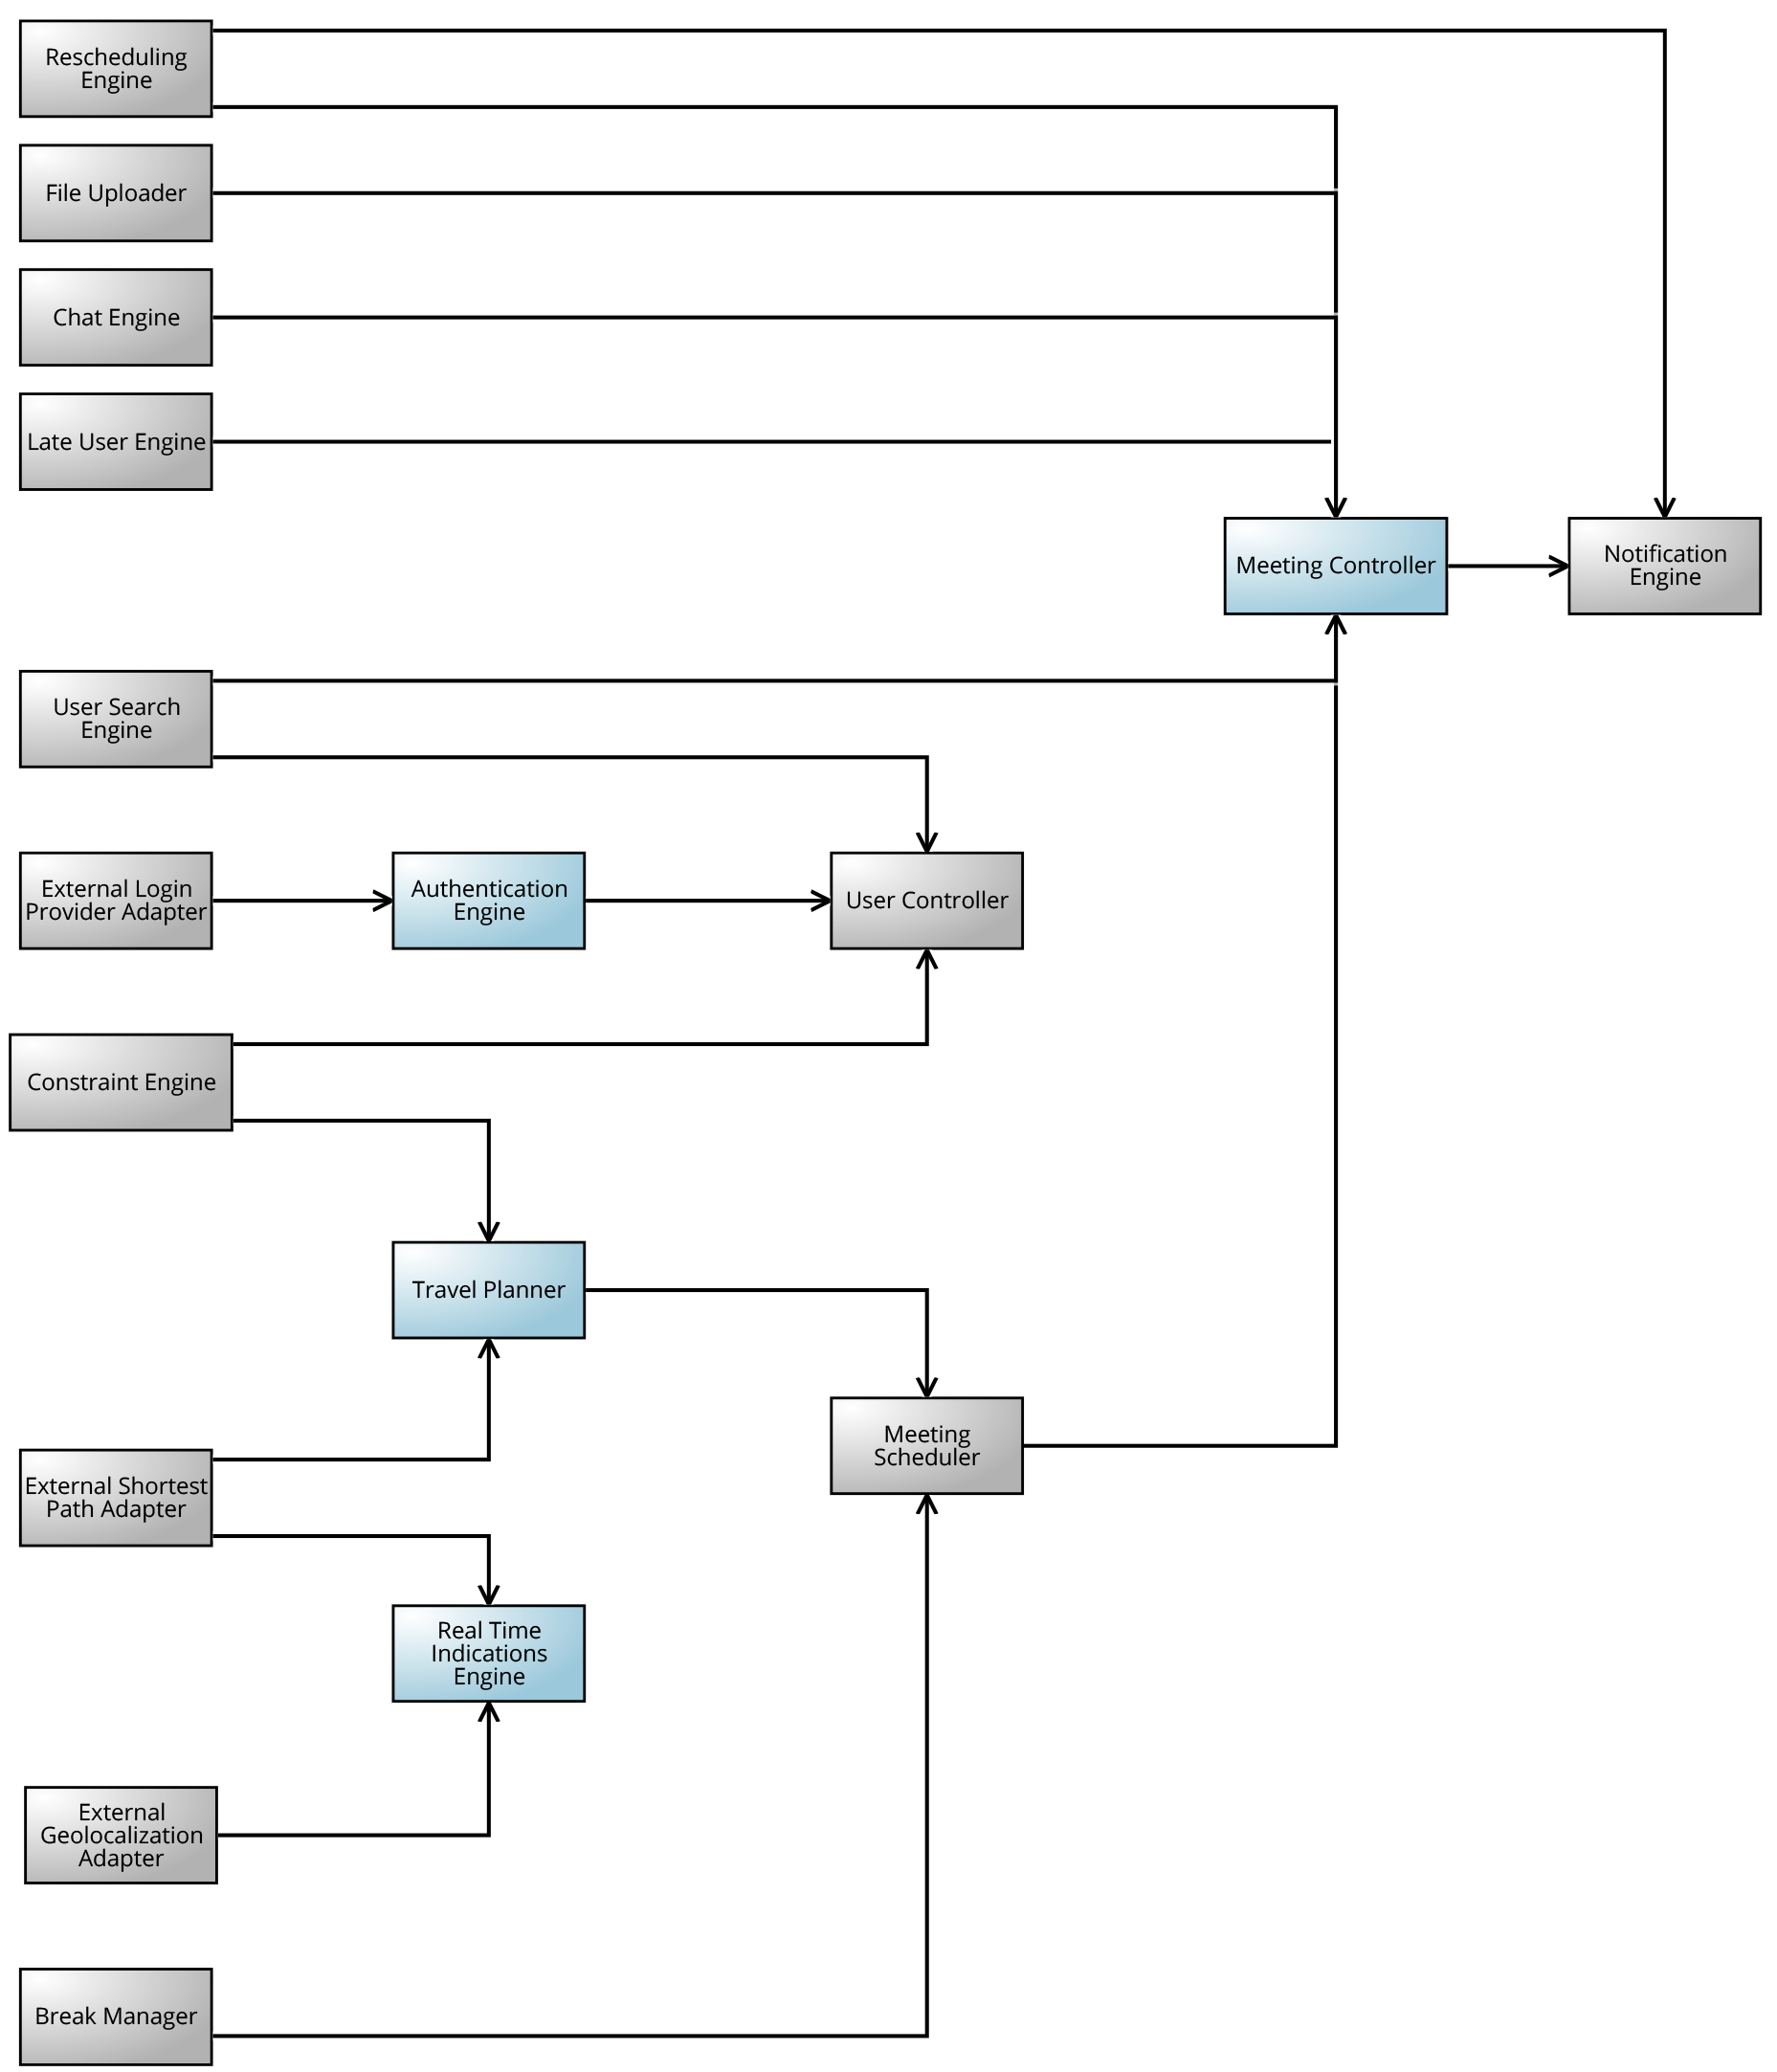
\includegraphics[scale = 0.22]{Images/UMLDiagrams/DependencyDiagramColored.png}
	\caption{Component Dependency Diagram}
\end{figure}

For this reason the best way to complete \projectname~ project is:
\begin{itemize}
	\item Develop Constraint Engine, External Shortest Path Adapter and Break Manager in parallels in order to have a complete background for the future development of other components.
	\item Develop all the Travel Planner component and integrate it with Constraint Engine and External Shortest Path Adapter following the integration test of the next chapters.
	\item Develop the Meeting Controller component. Since it is the most important component of the system, it is possible to implement it defying exactly the interfaces needed. Than, all the other components must be created such as they fit properly with the interfaces chosen by the Meeting Controller. 
	\item Develop Meeting Scheduler component and test it. Integrate it with the Travel Planner and the Meeting Controller component. After this process the main functionality of the system (i.e. organize daily schedule) should be completed. This must be tested properly.
	\item Develop External Login Adapter followed by the Authentication Engine and integrate it testing login and registration process.
	\item Develop User Search Engine and integrate it with Meeting Controller component.
	\item Develop User Controller, test it and integrate it with User Search Engine, Constraint Engine and Authentication Engine. After this process all the features related with user profile must be completed.
	\item Develop Reschedule Engine and integrate it with Meeting Controller.
	\item Develop Notification Engine and integrate it with the other components. This process must be tested properly .
	\item Develop all the features related with Meeting Controller such as File Uploader, Chat Engine and Late User Engine and integrate it with Meeting Controller, paying attention to fit with interfaces previously chosen by Meeting Controller component.
\end{itemize}
All the developing and integration processes must be immediately followed by their test.
After this process the system is completed with all its funciotnalites..... COLORARE IL DIAGRAMMA

\clearpage